\chapter{Solar Radiation Reflected from Exterior Surfaces}\label{solar-radiation-reflected-from-exterior-surfaces}

EnergyPlus has an option to calculate beam and sky solar radiation that is reflected from exterior surfaces and then strikes the building. This calculation occurs if ``withReflections'' is used on the SolarDistribution option in the Building object. For zones with detailed daylighting, these reflections are also considered in the daylight illuminance calculations.\footnote{A different method from that described here is used for calculating reflections from daylighting shelves (see ``Daylighting Shelves'').}

The reflecting surfaces fall into three categories:

\begin{itemize}
\item
  \textbf{Shadowing surfaces}. These are surfaces like overhangs or neighboring buildings entered with objects Shading:Site:Detailed, Shading:Building:Detailed, or Shading:Zone:Detailed Examples are shown in Figure~\ref{fig:examples-of-solar-reflection-from-shadowing}.

These surfaces can have diffuse and/or specular (beam-to-beam)~ reflectance values that are specified with the ShadingProperty:Reflectance object.

\item
  \textbf{Exterior building surfaces}. In this case one section of the building reflects solar radiation onto another section (and vice-versa). See Figure~\ref{fig:solar-reflection-from-building-surfaces-onto}.

Opaque building surfaces (walls, for example) are assumed to be diffusely reflecting. Windows and glass doors are assumed to be specularly reflecting. The reflectance values for opaque surfaces are calculated by the program from the Solar Absorptance and Visible Absorptance values of the outer material layer of the surface's construction. The reflectance values for windows and glass doors are calculated by the program from the reflectance properties of the individual glass layers that make up surface's construction assuming no shading device is present and taking into account inter-reflections among the layers.

\item
  \textbf{The ground surface}. Beam solar and sky solar reflection from the ground is calculated even if ``withReflections'' is not used (the default). But in this case the ground plane is considered unobstructed, i.e., the shadowing of the ground by the building itself or by obstructions such as neighboring buildings is ignored. This shadowing is taken into account only if ``WithReflections'' is used in the Solar Distribution field (in ``Building'' input object) (Figure~\ref{fig:shadowing-by-the-building-itself-affects-beam}). In this case the user-input value of ground view factor is not used.
\end{itemize}

\begin{figure}[hbtp] % fig 50
\centering
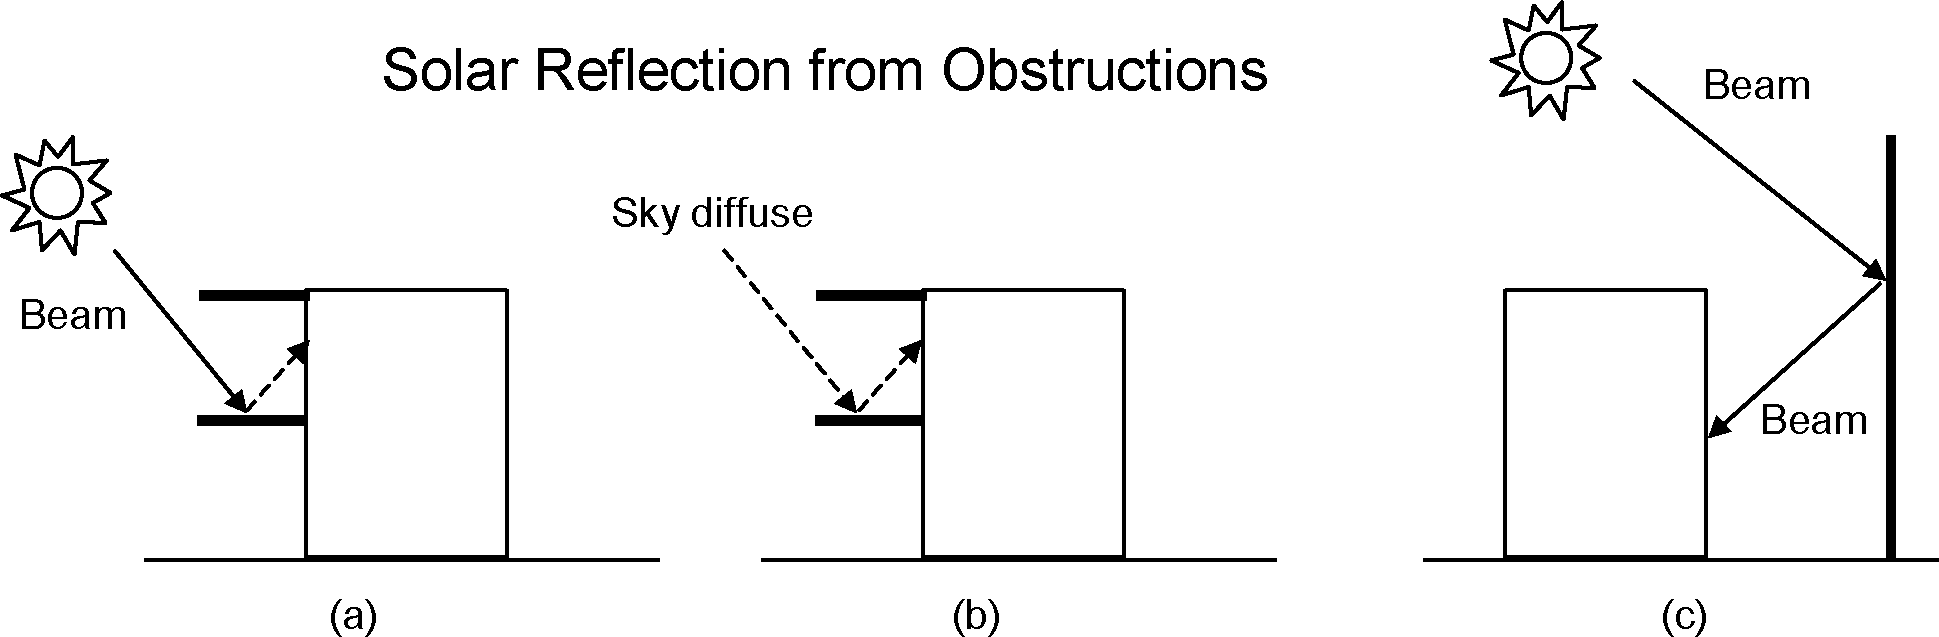
\includegraphics[width=0.9\textwidth, height=0.9\textheight, keepaspectratio=true]{media/image670.png}
\caption{Examples of solar reflection from shadowing surfaces in the Shading series of input objects. Solid arrows are beam solar radiation; dashed arrows are diffuse solar radiation. (a) Diffuse reflection of beam solar radiation from the top of an overhang. (b) Diffuse reflection of sky solar radiation from the top of an overhang. (c) Beam-to-beam (specular) reflection from the facade of an adjacent highly-glazed building represented by a vertical shadowing surface. \protect \label{fig:examples-of-solar-reflection-from-shadowing}}
\end{figure}

\begin{figure}[hbtp] % fig 51
\centering
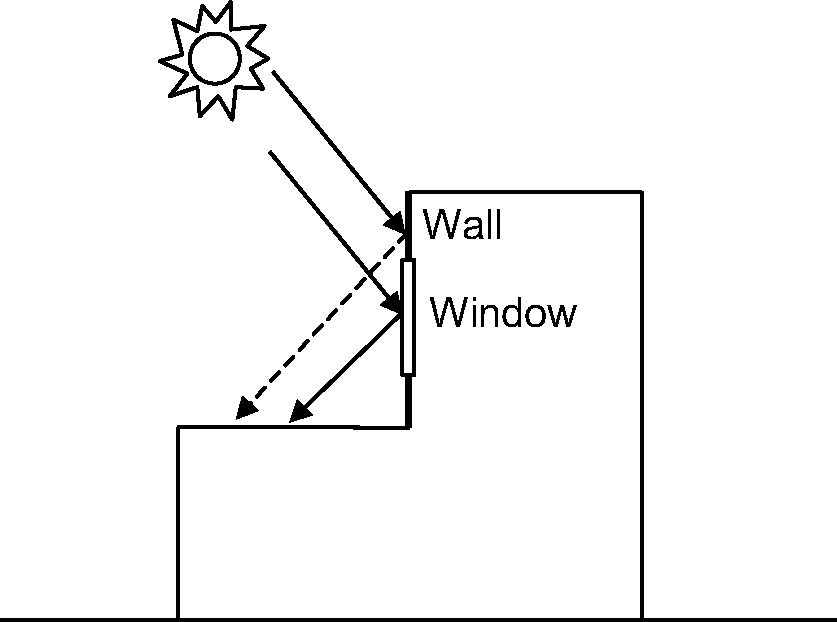
\includegraphics[width=0.9\textwidth, height=0.9\textheight, keepaspectratio=true]{media/image671.png}
\caption{Solar reflection from building surfaces onto other building surfaces. In this example beam solar reflects from a vertical section of the building onto a roof section. The reflection from the window is specular. The reflection from the wall is diffuse. \protect \label{fig:solar-reflection-from-building-surfaces-onto}}
\end{figure}

\begin{figure}[hbtp] % fig 52
\centering
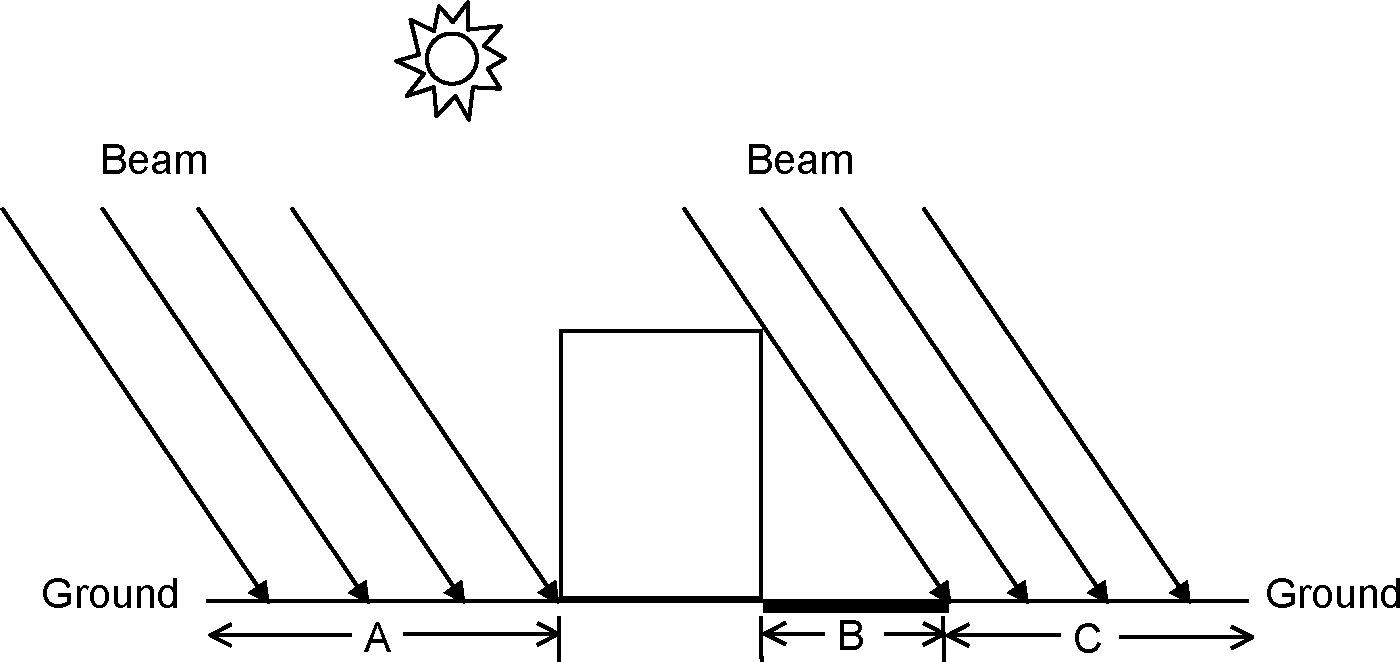
\includegraphics[width=0.9\textwidth, height=0.9\textheight, keepaspectratio=true]{media/image672.png}
\caption{Shadowing by the building itself affects beam solar reflection from the ground. Beam-to-diffuse reflection from the ground onto the building occurs only for sunlit areas, A and C, not for shaded area, B. Shadowing by the building also affects sky solar reflection from ground (not shown). \protect \label{fig:shadowing-by-the-building-itself-affects-beam}}
\end{figure}
